\startappendix{Additional Information}
\label{chapter:appendix}
Detailed data value for Figure \ref{fig:5.4}
\begin{eqnarray} 
\resizebox{0.9\linewidth}{!}{$
\begin{bmatrix}
0& 0& 0& 0& 0& 0& 0& 0& 0& 0& 0& 0.299586& 0& 0& 0& 0& 0& 0\\
0& 0& 0& 0.664053& 0& 0& 0& 0& 0& 0& 0& 0& 0& 0& 0& 0& 0& 0\\
0& 0& 0& 0& 0& 0& 0& 0& 0& 0& 0& 0& 0& 0& 0& 0& 0.021196& 0\\
0& 0& 0& 0& 0& 0& 0& 0& 0.00662804& 0& 0& 0& 0& 0& 0& 0& 0& 0\\
0& 0& 0& 0& 0& 0& 0& 0& 0& 0& 0& 0& 0.000642609& 0& 0& 0& 0& 0\\
0& 0& 0& 0& 0& 0& 0& 0& 0& 0& 0& 0& 0.00789& 0& 0& 0& 0& 0
\end{bmatrix}
$}
\end{eqnarray}

Detailed data value for Figure \ref{fig:5.5}
\begin{eqnarray}
\resizebox{0.9\linewidth}{!}{$
\begin{bmatrix}
0& 0& 0& 0& 0& 0& 0.299586& 0& 0& 0& 0& 0& 0& 0& 0& 0& 0& 0\\
0& 0& 0& 0.664053& 0& 0& 0& 0& 0& 0& 0& 0& 0& 0& 0& 0& 0& 0\\
0& 0.021196& 0& 0& 0& 0& 0& 0& 0& 0& 0& 0& 0& 0& 0& 0& 0& 0\\
0& 0& 0& 0& 0& 0& 0& 0& 0.00662804& 0& 0& 0& 0& 0& 0& 0& 0& 0\\
0& 0& 0& 0& 0& 0.000642609& 0& 0& 0& 0& 0& 0& 0& 0& 0& 0& 0& 0\\
0& 0& 0& 0& 0& 0.00789& 0& 0& 0& 0& 0& 0& 0& 0& 0& 0& 0& 0
\end{bmatrix}
$}
\end{eqnarray}

Detailed data value for Figure \ref{fig:5.6}
\begin{eqnarray}
\resizebox{0.9\linewidth}{!}{$
\begin{bmatrix}
0& 0& 0& 0& 0& 0& 0& 0& 0& 0& 0& 0.299586& 0& 0& 0& 0& 0& 0\\
0& 0& 0& 0.664053& 0& 0& 0& 0& 0& 0& 0& 0& 0& 0& 0& 0& 0& 0\\
0& 0& 0& 0& 0& 0& 0& 0& 0& 0& 0& 0& 0& 0& 0& 0& 0.021196& 0\\
0& 0& 0& 0& 0& 0& 0& 0& 0.00662804& 0& 0& 0& 0& 0& 0& 0& 0& 0\\
0& 0& 0& 0& 0& 0& 0& 0& 0& 0& 0& 0& 0.000642609& 0& 0& 0& 0& 0\\
0& 0& 0& 0& 0& 0& 0& 0& 0& 0& 0& 0& 0.00789& 0& 0& 0& 0& 0
\end{bmatrix}
$}
\end{eqnarray}


Detailed data value for Figure \ref{fig:6.1}
\begin{eqnarray}
\resizebox{0.5\linewidth}{!}{$
\begin {bmatrix}
0& 0& 0& 0& 0& 0& 0& 0.03218& 0 \\
0& 0.73929& 0& 0& 0& 0& 0& 0& 0 \\
0& 0& 0& 0.19745& 0& 0& 0& 0& 0 \\
0.00173& 0& 0& 0& 0& 0& 0& 0& 0 \\
0& 0& 0& 0& 0& 0& 0& 0.01819& 0 \\ 
0& 0& 0& 0& 0& 0& 0.01116& 0& 0
\end {bmatrix} 
$}
\label{eqn:7.4}
\end{eqnarray}

Detailed data value for Figure \ref{fig:6.2}
\begin{eqnarray}
\resizebox{0.5\linewidth}{!}{$
\begin {bmatrix}
0& 0& 0& 0& 0& 0& 0& 0.019308& 0 \\
0& 0.443574& 0& 0& 0& 0& 0& 0& 0 \\
0& 0& 0& 0.11847& 0& 0& 0& 0& 0  \\
0.001038& 0& 0& 0& 0& 0& 0& 0& 0 \\ 
0& 0& 0& 0& 0& 0& 0& 0.010914& 0 \\
0& 0& 0& 0& 0& 0& 0.006696& 0& 0 \\
0.4
\end {bmatrix}
$}
\label{eqn:7.5}
\end{eqnarray}

Detailed data value for Figure \ref{fig:6.4}. Target composition
\begin{eqnarray}
\resizebox{0.9\linewidth}{!}{$
\begin {bmatrix}
& 0& 0& 0& 0& 0.53762& 0& 0& 0& 0& 0& 0& 0& 0& 0& 0& 0& 0 \\
0& 0& 0.26894& 0& 0& 0& 0& 0& 0& 0& 0& 0& 0& 0& 0& 0& 0& 0 \\
0& 0& 0& 0& 0& 0& 0& 0& 0& 0& 0.03951& 0& 0& 0& 0& 0& 0& 0 \\
0& 0& 0& 0& 0& 0& 0& 0& 0& 0& 0& 0& 0& 0& 0& 0.11382& 0& 0 \\ 
0& 0& 0& 0& 0.01604& 0& 0& 0& 0& 0& 0& 0& 0& 0& 0& 0& 0& 0 \\
0& 0& 0.02407& 0& 0& 0& 0& 0& 0& 0& 0& 0& 0& 0& 0& 0& 0& 0 \\
\end {bmatrix}
$}
\label{eqn:7.}
\end{eqnarray}

Detailed data value for Figure \ref{fig:6.5}. Return composition of Result 2
\begin{eqnarray}
\resizebox{0.9\linewidth}{!}{$
\begin {bmatrix}
0& 0& 0& 0& 0& 0.414239& 0& 0& 0& 0& 0& 0& 0& 0& 0& 0& 0& 0 \\
0& 0& 0.20722& 0& 0& 0& 0& 0& 0& 0& 0& 0& 0& 0& 0& 0& 0& 0 \\ 
0& 0& 0& 0& 0& 0& 0& 0.0304427& 0& 0& 0& 0& 0& 0& 0& 0& 0& 0 \\
0& 0& 0.0876989& 0& 0& 0& 0& 0& 0& 0& 0& 0& 0& 0& 0& 0& 0& 0 \\
0& 0& 0& 0& 0.0123589& 0& 0& 0& 0& 0& 0& 0& 0& 0& 0& 0& 0& 0 \\
0& 0& 0.0185461& 0& 0& 0& 0& 0& 0& 0& 0& 0& 0& 0& 0& 0& 0& 0 \\
0.229495& 0& 0& 0& 0& 0& 0& 0& 0& 0& 0& 0& 0& 0& 0& 0& 0& 0 \\
\end {bmatrix}
$}
\label{eqn:7.}
\end{eqnarray}

Detailed data value for Figure \ref{fig:6.6}. Return composition of Result 6
\begin{eqnarray}
\resizebox{0.9\linewidth}{!}{$
\begin {bmatrix}
0& 0& 0& 0& 0& 0.27162& 0& 0& 0& 0& 0& 0& 0.142619& 0& 0& 0& 0& 0 \\
0& 0& 0.135875& 0& 0& 0& 0& 0& 0& 0& 0& 0& 0& 0& 0& 0.0713442& 0& 0 \\ 
0& 0& 0& 0& 0& 0& 0& 0.0104812& 0& 0& 0.0199615& 0& 0& 0& 0& 0& 0& 0 \\
0& 0& 0.0301941& 0& 0& 0& 0& 0& 0& 0& 0& 0& 0& 0& 0& 0.0575048& 0& 0 \\
0& 0& 0& 0& 0.00810383& 0& 0& 0& 0& 0& 0& 0& 0& 0.00425508& 0& 0& 0& 0 \\
0& 0& 0.0121608& 0& 0& 0& 0& 0& 0& 0& 0& 0& 0& 0& 0& 0.00638527& 0& 0 \\ 
0.229495& 0& 0& 0& 0& 0& 0& 0& 0& 0& 0& 0& 0&0& 0& 0& 0& 0 \\
\end {bmatrix}
$}
\label{eqn:7.}
\end{eqnarray}
%$g1 0.863411197459 g2 0.770505232571 g3 0.239946797277$


\begin{figure}[!ht] 
\centering
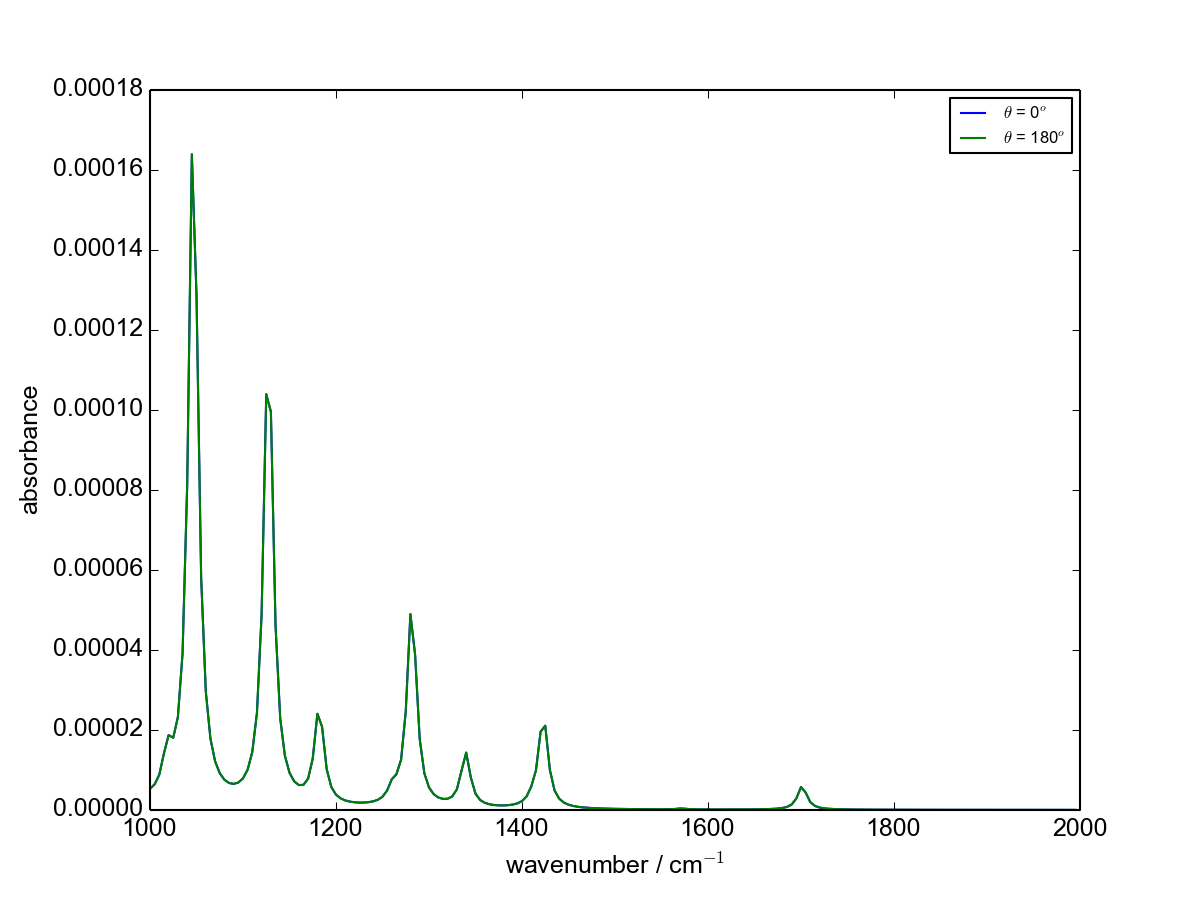
\includegraphics[scale=0.7]{Figures/Ala_candidates_plotting_ir_z_2.png}
\caption{IR $z$ projection spectrum for alanine candidate with $\theta$ of $0^{\circ}$ is identical to alanine candidate with $\theta$ of $180^{\circ}$} \label{fig:A.1}
\end{figure}

\begin{figure}[!ht] 
\centering
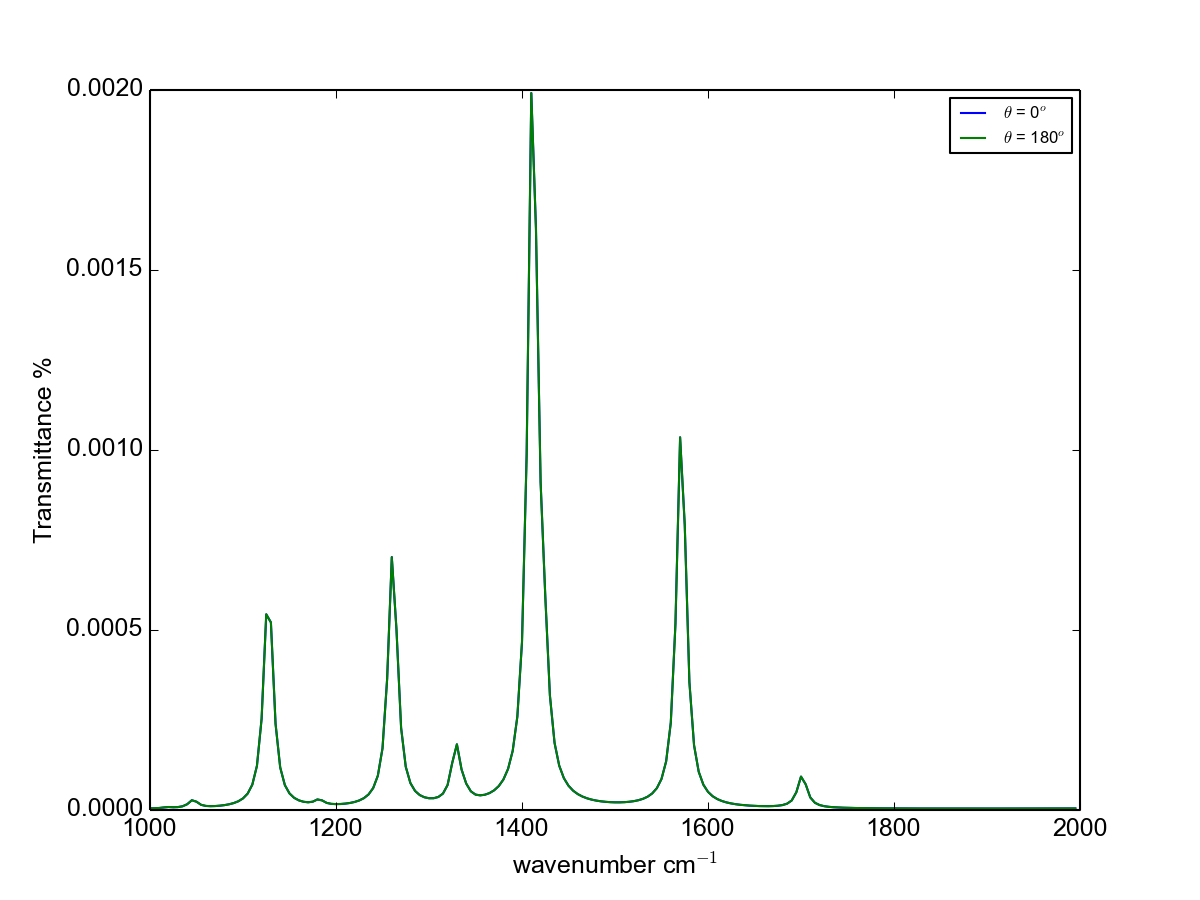
\includegraphics[scale=0.7]{Figures/Ala_candidates_plotting_raman_zz_2.png}
\caption{Raman $zz$ projection spectrum for alanine candidate with $\theta$ of $0^{\circ}$ is identical to alanine candidate with $\theta$ of $180^{\circ}$} \label{fig:A.2}
\end{figure}

\begin{figure}[!ht] 
\centering
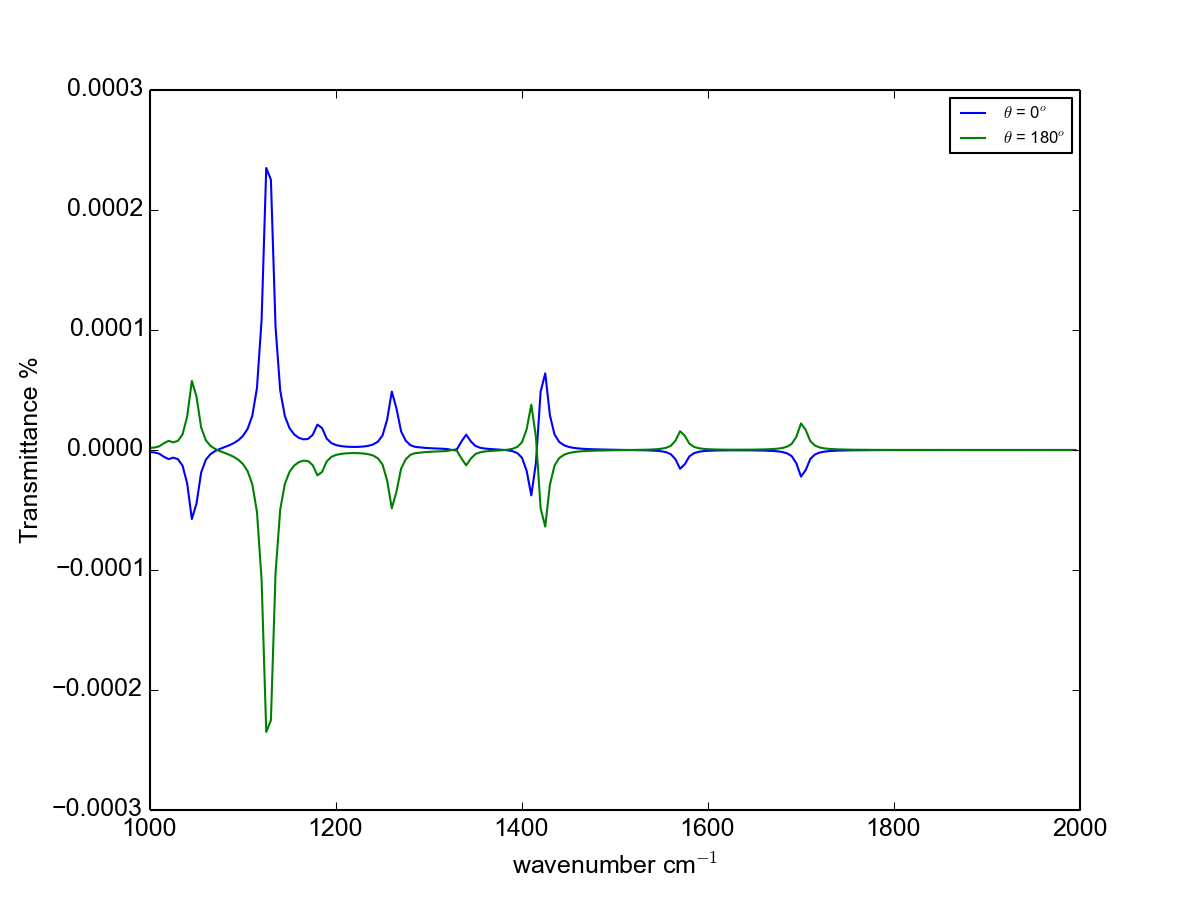
\includegraphics[scale=0.7]{Figures/Ala_candidates_plotting_sfg_zzz_2.png}
\caption{SFG $zzz$ projection spectrum for alanine candidate with $\theta$ of $0^{\circ}$ is not identical to alanine candidate with $\theta$ of $180^{\circ}$, but symmetric along wavelength} 
\label{fig:A.3}
\end{figure}
